 \chapter{Experimentation and Analysis\label{ch:Experimentation and Analysis}}

This chapter is intended to provide the experimental proof of the proposed extension of the previously formulated algorithm from \cite{ref5}. Through this chapter, the detailed explanation of the additional constraints that are added to the unoptimized algorithm from the previous chapter is provided. Next micro and macro agent simulations are presented pertaining to certain cases and scenarios to compare between the unoptimized and the optimized algorithms. The resulting observations and statistics are then presented for further analysis and the implications are then discussed.

\section{Optimization through Constraints}
\label{sec: Optimization through Constraints}

From the equations \ref{eq1}, \ref{eq2} and \ref{eq3}, the basic conditions for agent occupancy, flow control and cell capacity is discussed. However these conditions are hardly realistic when compared to modelling a real crowd of agents. In realistic scenarios, groups of people have altered behavior, confusion panic etc. There will be different forms of social constraints, varying movement speeds, and due to the impaired cognition, perceptions can change leading to different decisions that are made during a catastrophe. To model some of these realistic scenarios, it became evident that the inclusion of certain more properties to the scenario was mandatory. The following conditions as mentioned in section \ref{sec:intro:Objectives and Approach} is analyzed here:

\begin{enumerate}
  \item Cell capacity specification by defining social distances
  \begin{itemize}
  	\item Although PedSim comes by default with a cell class, it does not go coherently with the topology, as cell divisions are highly subjective and can change their length and breadth according to the defined scenario. To cater for this, manipulation of the social forces constraint causes agents to maintain a certain "social distance" from each other. This can be used to our advantage to simulate cell capacities based on these social distances.
  \end{itemize}
  \item Definition of total area capacity and doors flow capacity constraints -congestion control
  \begin{itemize}
  	\item The algorithm presented in section \ref{sec: Algorithm Description} unfortunately does not handle congestion as well as the proposed algorithm due to the simplistic constraints present. Providing additional constraint for area capacity, door flow capacity and passageway capacity can help reduce congestion and enable the re-routing of agents to alternate exits or routes in real time.
  \end{itemize}
  \item Simulating social attachment among some agents
  \begin{itemize}
  	\item With the introduction of the group constraint, social attachments can be modeled for a more realistic approach. For instance friends move together, a mother will most likely not be separable from her child etc. These groups can be defined during the simulation and then observed for the various real time decisions that these groups of agents make.
  \end{itemize}
  \item Setting the speed accordingly for various groups
  \begin{itemize}
  	\item By default PedSim models for microscopic agents and hence the entirety of the agents are considered as a single group. The movement speed for these agents are varied across a distribution and the average speed set for the microscopic group of agents. By setting a variable speed constraint and with the introduction of groups, we model PedSim to cater for macro and micro agent simulation and thus support varying speeds according to the different group formations that can be defined during the simulation. In other words $v_{max}$ is not fixed across all agents.
  \end{itemize}
\end{enumerate}

The PedSim library is extended to be inclusive of the algorithm from the section \ref{sec: Algorithm Description} and the aforementioned constraints in order to simulate the various scenarios for micro and macro agents. The following section provides a detailed analysis of the various scenarios that are simulated within the PedSim environment.  

\section{Simulation and Scenario Analysis}
\label{sec: Simulation and Scenario Analysis}

This section contains the experimental analysis based on the scenarios that are presented in the forthcoming subsections. It must be noted that the following simulations are run on a PC with the following specifications - Ubuntu 18.04, 8 GB ram, and an i5 processor with 2.5 ghz clock speed. A series of sub-sections are present in this section - each representing a particular scenario for simulation. The scenario will be described and the corresponding tabular observations and graph is then presented. 

There are some properties that are common to scenarios. We follow similar topological constraints as given in \cite{ref5}. For instance, in the previous work presented, the cells are assumed to be isometric, i.e. the cells are bi-directional and can be crossed from any direction with the same amount of time. In the scenarios presented, the cells are assumed to be isometric as well.

According to the work by Daamen et al. \cite{ref23}, door capacities are presented, where they are based on varying stress and composition levels of agents and he subesquently proposes an average of 2.8 persons per second for a 1 meter wide door $(p/m/s)$. In order to perform a statistical analysis and to remain coherent with the results with from \cite{ref5}, the door capacities and cell capacities are modeled after the presented stats in the aforementioned work. In \cite{ref5} the pessimistic and optimistic values considered are 1.03 $p/m/s$ and 3.23 $p/m/s$ respectively. This translates to a maximum of 5 people in pessimistic and a maximum of 16 people in optimistic situation can pass through a 1 meter wide door per slot time (5 seconds). Hence the same values will be considered here as well. There are also a certain terms that are used in this section, namely, optimistic and pessimistic. Optimistic scenario assumes that no passageways and exits are blocked. Whereas pessimistic scenario assumes that 50\% of the emergency exits are blocked and passageways can accommodate only 5 people at a time. 

The maximum number of people considered is 1008, as mentioned in \cite{ref5}. All the above conditions are compliant with the mentioned paper.

\subsection{Case 1: Macro Agent Simulation Comparing Optimized and Un-Optimized Algorithms}
\label{sec: Case 1: Macro Agent Simulation Comparing Optimized and Un-Optimized Algorithms}

The first case is depicts the CPU run time comparison between macro agents(single or no group concept is present here) that follow the un-optimized algorithm from \cite{ref5} and the proposed extension of the mentioned algorithm. For the current scenario, pessimistic path scenario is incorporated in order to keep the coherency of results and perform the necessary comparisons with the aforementioned paper.

A total of 1008 people are taken for the purposes of this simulation. Various walking speed scenarios among acquintances and friendly dyads are presented in the work by Wagnild et al. \cite{ref24}, however since there are no complex group formations that are currently part of the simulation, the speed of 1.2 $m/s$ estimated in J. Ye's average \textit{free flowing walking velocity} \cite{ref25} is used here.

The original code for simulation was written on OPL language and solved on CPLEX version 12.8.0 \cite{ref5}. However codebase for the modified algorithm has since been translated to the PedSim environment. The following table \ref{Macro Agent Simulation - Optimized vs UnOptimized Algorithm} represents the simulation times between the optimized and the un-optimized algorithms.
 

\begin{table}[H]
\centering
\begin{adjustbox}{angle=270}
\scalebox{0.7}{
\begin{tabular}{|l|l|l|l|l|l|l|l|} 
\hline
\textcolor[rgb]{0.133,0.133,0.133}{τ} & Evacuees & CPU Time (sec) - Optimized & CPU Time (sec) - Un-Optimized & \textcolor[rgb]{0.133,0.133,0.133}{τ} & Evacuees & CPU Time (sec) - Optimized & CPU Time (sec) - Un-Optimized  \\ 
\hline
1                                     & 20       & 0.25                       & 0.28                         & 27                                    & 540      & 4.9                        & 2.61                          \\
2                                     & 40       & 0.28                       & 0.31                         & 28                                    & 560      & 5.1                        & 2.77                          \\
3                                     & 60       & 0.47                       & 0.44                         & 29                                    & 580      & 5.7                        & 2.84                          \\
4                                     & 80       & 0.61                       & 0.53                         & 30                                    & 600      & 6                          & 2.96                          \\
5                                     & 100      & 0.63                       & 0.47                         & 31                                    & 620      & 6.5                        & 3.1                           \\
6                                     & 120      & 0.69                       & 0.58                         & 32                                    & 640      & 6.94                       & 3.53                          \\
7                                     & 140      & 0.72                       & 0.6                          & 33                                    & 660      & 7.2                        & 3.32                          \\
8                                     & 160      & 0.75                       & 0.61                         & 34                                    & 680      & 7.76                       & 3.54                          \\
9                                     & 180      & 0.82                       & 0.71                         & 35                                    & 700      & 7.96                       & 3.91                          \\
10                                    & 200      & 0.88                       & 0.76                         & 36                                    & 720      & 8.4                        & 3.42                          \\
11                                    & 220      & 1.1                        & 0.83                         & 37                                    & 740      & 8.7                        & 4.14                          \\
12                                    & 240      & 1.22                       & 0.88                         & 38                                    & 760      & 9.3                        & 4.16                          \\
13                                    & 260      & 1.27                       & 1.01                         & 39                                    & 780      & 9.88                       & 4.17                          \\
14                                    & 280      & 1.33                       & 1.09                         & 40                                    & 800      & 10.4                       & 4.19                          \\
15                                    & 300      & 1.4                        & 1.12                         & 41                                    & 820      & 10.79                      & 4.3                           \\
16                                    & 320      & 1.6                        & 1.44                         & 42                                    & 840      & 11.5                       & 5.13                          \\
17                                    & 340      & 1.82                       & 1.28                         & 43                                    & 860      & 12.37                      & 5.07                          \\
18                                    & 360      & 1.99                       & 1.33                         & 44                                    & 880      & 13.01                      & 5.12                          \\
19                                    & 380      & 2.1                        & 1.57                         & 45                                    & 900      & 13.68                      & 5.27                          \\
20                                    & 400      & 2.3                        & 1.61                         & 46                                    & 920      & 14.5                       & 5.36                          \\
21                                    & 420      & 2.44                       & 1.73                         & 47                                    & 940      & 15.4                       & 5.49                          \\
22                                    & 440      & 2.6                        & 1.88                         & 48                                    & 960      & 16.04                      & 6.01                          \\
23                                    & 460      & 2.9                        & 2.02                         & 49                                    & 980      & 17.07                      & 6.35                          \\
24                                    & 480      & 3.3                        & 2.08                         & 50                                    & 1000     & 18.2                       & 6.25                          \\
25                                    & 500      & 3.8                        & 2.19                         & 51                                    & 1008     & 19.4                       & 6.47                          \\
26                                    & 520      & 4.4                        & 2.35                         &                                       &          &                            &                               \\
\hline
\end{tabular}}
\end{adjustbox}
\caption{Macro Agent Simulation - Optimized vs UnOptimized Algorithm}
\label{Macro Agent Simulation - Optimized vs UnOptimized Algorithm}
\end{table}

It should be mentioned that for the purposes of proper identication between the two scenarios in comparison, the simulation that runs with the constraints on the base algorithm is said to be running an optimized algorithm whereas the simulation without these constraints is said to be running on an un-optimized algorithm. 

It is evident from the above figure that the optimized algorithm takes an exponential time to compute the simulation times for the macro agents at the given number of time steps. Below is a graphical description of the observed statistical values from the table \ref{Macro Agent Simulation - Optimized vs UnOptimized Algorithm}.

\begin{figure}[H]
  \centering
  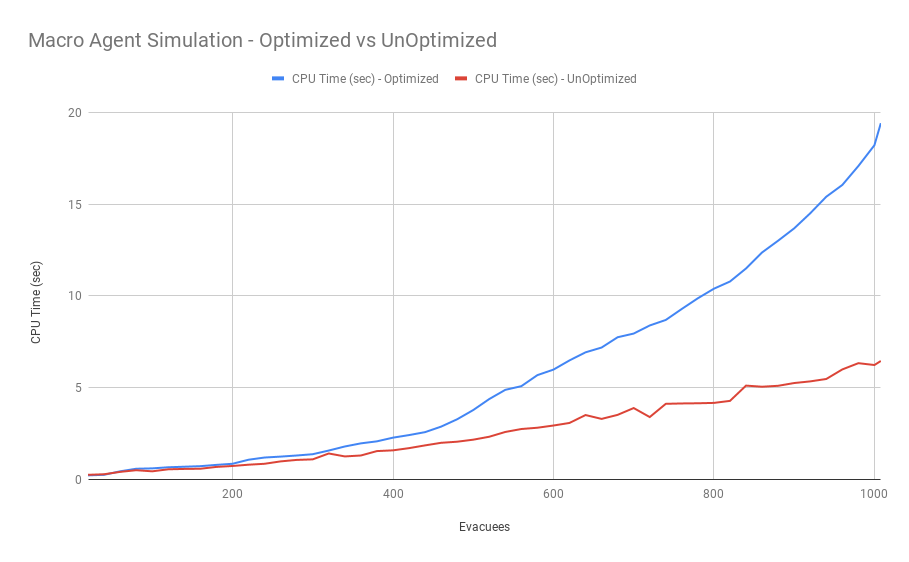
\includegraphics[scale=0.5]{simulation/Macro_Agent_Simulation.png}
  \caption{Macro Agent Simulation - Optimized vs UnOptimized Algorithms}
  \label{Macro Agent Simulation}
\end{figure}

The above figure \ref{Macro Agent Simulation} depicts the difference in the performance experienced as the constraints placed are higher in count and complexity. In the present scenario, not all the constraints are incorporated however. In macro agent simulation, no grouping is employed, hence there is no grouping constraint. This in turn also affects the varying speed constraint as groups of agents are not involved. It is also noteworthy mentioning that single agents can be considered as individual groups as well. Since there is no such constraint, the average of 1.2 $m/s$ velocity for all agents is applied and the simulation of the agents are then performed.


\subsection{Case 2: Run Time Comparison between Micro and Macro Agent Simulation}
\label{sec: Case 2: Run Time Comparison between Micro and Macro Agent Simulation}

This case is similar in terms of objective to the previous case \ref{sec: Case 1: Macro Agent Simulation Comparing Optimized and Un-Optimized Algorithms}. However the key difference lies in what is compared in this particular scenario. Micro and macro agent simulation scenarios are compared in this case. Since there is micro agents that are also included, grouping constraints are included and subsequently varying velocities based on grouping and affiliation.

According to the work by Wagnild et al. \cite{ref24}, walking speeds are highly depend on the company and the lowest speed of the person present in the group. This scenario is inclusive of group constraints. However this scenario is also only to compare the actual running times of the simulated output. Complexities regarding group dynamics are not compared here. To keep the results coherent, the macro agents are considered with the uniform speed as mentioned in the previous section. The micro agents consists of mixed groups and individuals. To keep group velocity diversity among the micro agents, 20\% of the total number of micro agents are randomly distributed with varying speeds between the range of 0.7 $m/s$ and 1.5 $m/s$.   

The comparison values are based off on the pessimistic path scenario as presented in \cite{ref5}. A cross way comparison between macro agents with un-optimized algorithm, macro agents simulated with optimized algorithm and micro agent with constraints is tabulated in the table below. The CPU run time values for the microscopic agents that are simulated using the un-optimzed are obtained from the charted values from table 2.0 from the aforementioned paper, based on which the other two comparisons can be made and analyzed.

A total number of evacuees upto 1008 are considered for the comparisons, similar to the previous section \ref{sec: Case 1: Macro Agent Simulation Comparing Optimized and Un-Optimized Algorithms}. 

\begin{table}
\centering
\begin{adjustbox}{angle=270}
\scalebox{0.7}{
\begin{tabular}{|l|l|l|l|} 
\hline
Evacuees & CPU Time (sec) - Micro Agent Sim:Optimized with Constraints & Evacuees & CPU Time (sec) - Micro Agent Sim:Optimized with Constraints  \\ 
\hline
20       & 0.4                                                         & 540      & 10.8                                                         \\
40       & 0.46                                                        & 560      & 11.5                                                         \\
60       & 0.6                                                         & 580      & 12.3                                                         \\
80       & 0.8                                                         & 600      & 13.8                                                         \\
100      & 0.9                                                         & 620      & 14.97                                                        \\
120      & 1.01                                                        & 640      & 15.92                                                        \\
140      & 1.11                                                        & 660      & 17.3                                                         \\
160      & 1.4                                                         & 680      & 19.2                                                         \\
180      & 1.7                                                         & 700      & 21.84                                                        \\
200      & 2                                                           & 720      & 23.7                                                         \\
220      & 2.3                                                         & 740      & 25.9                                                         \\
240      & 2.4                                                         & 760      & 27.9                                                         \\
260      & 2.7                                                         & 780      & 30.2                                                         \\
280      & 3.2                                                         & 800      & 33.5                                                         \\
300      & 3.5                                                         & 820      & 36.7                                                         \\
320      & 3.9                                                         & 840      & 39                                                           \\
340      & 4.3                                                         & 860      & 43.3                                                         \\
360      & 4.8                                                         & 880      & 47.2                                                         \\
380      & 5.4                                                         & 900      & 50.34                                                        \\
400      & 5.9                                                         & 920      & 54.2                                                         \\
420      & 6.5                                                         & 940      & 58.99                                                        \\
440      & 6.97                                                        & 960      & 64.2                                                         \\
460      & 7.6                                                         & 980      & 68.2                                                         \\
480      & 8.1                                                         & 1000     & 74.78                                                        \\
500      & 8.7                                                         & 1008     & 76.34                                                        \\
520      & 9.7                                                         &          &                                                              \\
\hline
\end{tabular}}
\end{adjustbox}
\caption{CPU Time Comparison between Micro and Macro Agent Simulation}
\label{CPU Time Comparison between Micro and Macro Agent Simulation}
\end{table}  

As it can be noted from the above table \ref{CPU Time Comparison between Micro and Macro Agent Simulation}, the time taken for the micro agent simulation far exceeds the time taken by both the previous simulations - for macro agent using both optimized and un-optimized algorithms. However, it should be noted that the micro agent simulation has 20\% of the entire participants at a reduced movement speed, during each simulation run. Since the number of reduced movement speed agents increase exponentially for each trial run, so does the computation time. These agents who have reduced speeds are also randomized to form certain affliate bonds and groups. 

More discussion on the nature of such groups and their implications are discussed in the next sub-section where the evacuation time is discussed in detail and simulations are run in order to observe the actual time taken due to the additional constraints.

The below figure \ref{Micro vs Macro Agent Simulation} represents the comparison between the 3 major simulation models and their exceedingly apparent ranges of computation times. 

\begin{figure}[H]
  \centering
  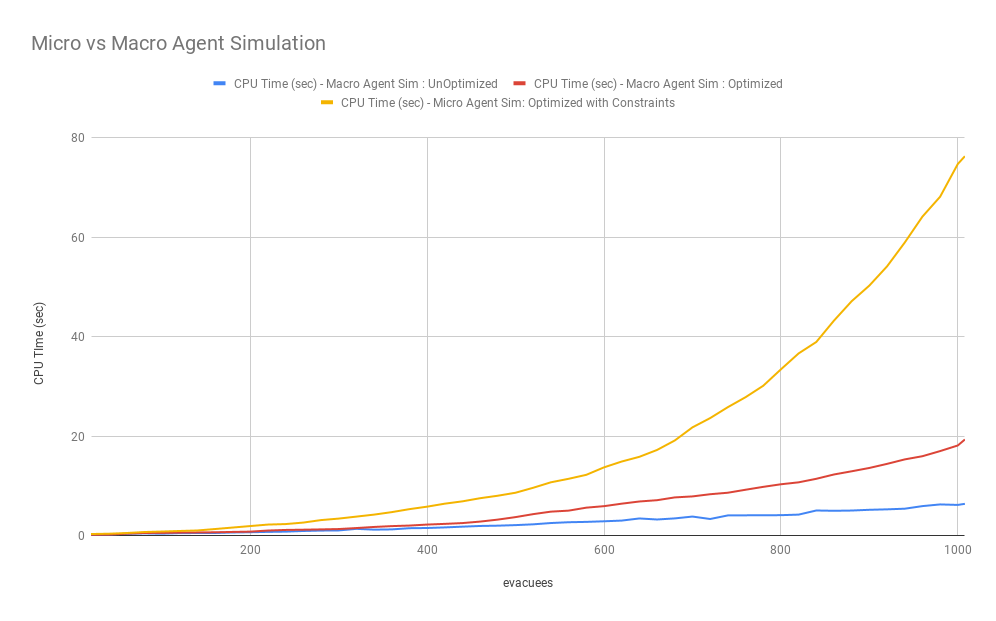
\includegraphics[scale=0.47]{simulation/Micro_vs_Macro_Agent_Simulation.png}
  \caption{Micro vs Macro Agent Simulation}
  \label{Micro vs Macro Agent Simulation}
\end{figure}

From the figure, the following inferences can be made:

\begin{enumerate}
  \item The macro agent simulation with no constraints and simulated according to the base algorithm and a constant $v_{max}$ movement velocity has a time complexity of $O(N)$.
  \item The macro agent simulation subjected to constraints such as social force definition, area capacity and flow capacity, exhibit a time complexity of $O(N^2)$.
  \item Micro agent simulation subjected to varying speeds and grouping in addition to social forces and flow capacity definition for congestion control, exhibit a time complexity of $O(N^3)$.
\end{enumerate}

The implications for these inferences will be discussed in section 4.3.


\subsection{Case 3: Congestion Dynamics and Flow Control}
\label{sec: Case 3: Congestion Dynamics and Flow Control}

This section presents a detailed case on the effect of the width of emergency exits on the evacuation time. The work by H. Muccini et al. \cite{ref5} focuses on an ideal and optimal path without accounting for more advanced constraints. One of the most important effects of a disaster on human agents is the element of chaos and panic. This causes most agents to panic and make rash decisions, all clustering towards an exit point. This causes massive congestions and jams which ultimately leads to stampedes and also the failure for the agents to evacuate to an exist point in the shortest time frame possible. To analyze an optimal egress path however, we do not simulate congestion itself as such, rather we aim for congestion avoidance. To avoid congestion, the routes for various people need to be calculated in real time in order to re-route in the case of an impending congestion scenario.

In order to analyze the congestion, we must first answer the question, what leads to congestion? The answer is two fold as follows:
\begin{itemize}
  \item The obvious answer is - too little space and too many people to fill that space. The forthcoming tables and graphs are to experiment the effect of exit width on congestion.
  \item The second answer is more complex, dealing with walking speeds, social forces and group decisions. 
\end{itemize}

In section \ref{sec: Case 4: Shortest Path vs Ideal Path}, detailed case study on walking speeds and decision making is presented. Although the same group dynamics applies to this case too, the focus is on exit width. The forthcoming tables and graph depict the various scenarios that are simulated for both macro and micro agents using the un-optimized and optimized algorithms respectively.

The following table \ref{Emergency Exits Width vs Evacuation Time : Optimistic Values for Macro Agent Model} depicts optimistic values for macro agents whilst varying exit capacities and thus in turn affecting flow dynamics.

\begin{table}[H]
\centering
\scalebox{0.7}{
\begin{tabular}{|l|l|l|} 
\hline
Emergency Exit Width (m) & \begin{tabular}[c]{@{}l@{}}Evacuation Time Horizon $(\tau)$ - \\Optimistic values for \\Unoptimized Algorithm\end{tabular} & \begin{tabular}[c]{@{}l@{}}Evacuation Time Horizon $(\tau)$ - \\Optimistic Values for \\Optimized Algorithm\end{tabular}  \\ 
\hline
0.4                      & 45                                                                                                                  & 83                                                                                                                 \\
0.5                      & 43                                                                                                                  & 79                                                                                                                 \\
0.6                      & 37                                                                                                                  & 76                                                                                                                 \\
0.7                      & 33                                                                                                                  & 73                                                                                                                 \\
0.8                      & 28                                                                                                                  & 70                                                                                                                 \\
0.9                      & 25                                                                                                                  & 68                                                                                                                 \\
1.0                      & 22                                                                                                                  & 62                                                                                                                 \\
1.1                      & 20                                                                                                                  & 58                                                                                                                 \\
1.2                      & 16                                                                                                                  & 53                                                                                                                 \\
1.3                      & 12                                                                                                                  & 48                                                                                                                 \\
1.4                      & 11                                                                                                                  & 45                                                                                                                 \\
1.5                      & 10                                                                                                                  & 40                                                                                                                 \\
1.6                      & 9                                                                                                                   & 37                                                                                                                 \\
1.7                      & 9                                                                                                                   & 32                                                                                                                 \\
1.8                      & 8                                                                                                                   & 29                                                                                                                 \\
1.9                      & 7                                                                                                                   & 25                                                                                                                 \\
2.0                      & 6                                                                                                                   & 20                                                                                                                 \\
2.1                      & 5                                                                                                                   & 18                                                                                                                 \\
2.2                      & 5                                                                                                                   & 15                                                                                                                 \\
2.3                      & 5                                                                                                                   & 12                                                                                                                 \\
2.4                      & 4                                                                                                                   & 8                                                                                                                  \\
2.5                      & 3                                                                                                                   & 6                                                                                                                  \\
2.6                      & 3                                                                                                                   & 5                                                                                                                  \\
2.7                      & 3                                                                                                                   & 3                                                                                                                  \\
2.8                      & 2                                                                                                                   & 2                                                                                                                  \\
2.9                      & 2                                                                                                                   & 2                                                                                                                  \\
3.0                      & 1                                                                                                                   & 1                                                                                                                  \\
\hline
\end{tabular}}
\caption{Emergency Exits Width vs Evacuation Time : Optimistic Values for Macro Agent Model}
\label{Emergency Exits Width vs Evacuation Time : Optimistic Values for Macro Agent Model}
\end{table}

Comparison between the pessimistic cases of optimized and the un-optimized cases are presented for macro agent model below in table \ref{Emergency Exits Width vs Evacuation Time : Pessimistic values for Macro Agent Simulation}:


\begin{table}[H]
\centering
\scalebox{0.7}{
\begin{tabular}{|l|l|l|} 
\hline
    Emergency Exit Width (m) & \begin{tabular}[c]{@{}l@{}}Evacuation Time Horizon $(\tau)$ -\\Pessimistic Values for \\UnOptimized Algorithm\end{tabular} & \begin{tabular}[c]{@{}l@{}}Evacuation Time Horizon $(\tau)$ -\\Pessimistic Values for \\Optimized Algorithm\end{tabular}  \\ 
\hline
0.4                      & 120                                                                                                                 & 205                                                                                                                \\
0.5                      & 105                                                                                                                 & 192                                                                                                                \\
0.6                      & 94                                                                                                                  & 181                                                                                                                \\
0.7                      & 86                                                                                                                  & 173                                                                                                                \\
0.8                      & 76                                                                                                                  & 163                                                                                                                \\
0.9                      & 68                                                                                                                  & 155                                                                                                                \\
1.0                      & 62                                                                                                                  & 140                                                                                                                \\
1.1                      & 56                                                                                                                  & 127                                                                                                                \\
1.2                      & 53                                                                                                                  & 111                                                                                                                \\
1.3                      & 48                                                                                                                  & 101                                                                                                                \\
1.4                      & 45                                                                                                                  & 93                                                                                                                 \\
1.5                      & 42                                                                                                                  & 80                                                                                                                 \\
1.6                      & 37                                                                                                                  & 72                                                                                                                 \\
1.7                      & 33                                                                                                                  & 65                                                                                                                 \\
1.8                      & 29                                                                                                                  & 52                                                                                                                 \\
1.9                      & 25                                                                                                                  & 47                                                                                                                 \\
2.0                      & 20                                                                                                                  & 30                                                                                                                 \\
2.1                      & 18                                                                                                                  & 19                                                                                                                 \\
2.2                      & 15                                                                                                                  & 17                                                                                                                 \\
2.3                      & 12                                                                                                                  & 14                                                                                                                 \\
2.4                      & 8                                                                                                                   & 11                                                                                                                 \\
2.5                      & 6                                                                                                                   & 8                                                                                                                  \\
2.6                      & 5                                                                                                                   & 6                                                                                                                  \\
2.7                      & 3                                                                                                                   & 5                                                                                                                  \\
2.8                      & 2                                                                                                                   & 3                                                                                                                  \\
2.9                      & 2                                                                                                                   & 2                                                                                                                  \\
3.0                      & 1                                                                                                                   & 1                                                                                                                  \\
\hline
\end{tabular}}
\caption{Emergency Exits Width vs Evacuation Time : Pessimistic values for Macro Agent Simulation}
\label{Emergency Exits Width vs Evacuation Time : Pessimistic values for Macro Agent Simulation}
\end{table}

To run a simulation for the case of micro model agents, certain characteristics were given to 20\% of the total number of agents in each case. The characteristics include variable speeds(random speed between 0. 7 $m/s$ and 1.4 $m/s$), and the other constraints of area capacity and the variable exit door capacity as follows:


\begin{table}[H]
\centering
\scalebox{0.7}{
\begin{tabular}{|l|l|l|} 
\hline
Emergency Exit Width (m) & \begin{tabular}[c]{@{}l@{}}Evacuation Time Horizon $(\tau)$ - \\Optimistic Values for \\Micro Agent Simulation\end{tabular} & \begin{tabular}[c]{@{}l@{}}Evacuation Time Horizon $(\tau)$ - \\Pessimistic Values for \\Micro Agent Simulation\end{tabular}  \\ 
\hline
0.4                      & 246                                                                                                                  & 415                                                                                                                    \\
0.5                      & 223                                                                                                                  & 370                                                                                                                    \\
0.6                      & 202                                                                                                                  & 340                                                                                                                    \\
0.7                      & 192                                                                                                                  & 306                                                                                                                    \\
0.8                      & 184                                                                                                                  & 292                                                                                                                    \\
0.9                      & 178                                                                                                                  & 270                                                                                                                    \\
1.0                      & 155                                                                                                                  & 240                                                                                                                    \\
1.1                      & 140                                                                                                                  & 212                                                                                                                    \\
1.2                      & 129                                                                                                                  & 193                                                                                                                    \\
1.3                      & 111                                                                                                                  & 163                                                                                                                    \\
1.4                      & 101                                                                                                                  & 140                                                                                                                    \\
1.5                      & 85                                                                                                                   & 124                                                                                                                    \\
1.6                      & 74                                                                                                                   & 112                                                                                                                    \\
1.7                      & 65                                                                                                                   & 99                                                                                                                     \\
1.8                      & 51                                                                                                                   & 83                                                                                                                     \\
1.9                      & 48                                                                                                                   & 60                                                                                                                     \\
2.0                      & 31                                                                                                                   & 47                                                                                                                     \\
2.1                      & 19                                                                                                                   & 33                                                                                                                     \\
2.2                      & 16                                                                                                                   & 28                                                                                                                     \\
2.3                      & 13                                                                                                                   & 20                                                                                                                     \\
2.4                      & 10                                                                                                                   & 16                                                                                                                     \\
2.5                      & 8                                                                                                                    & 9                                                                                                                      \\
2.6                      & 7                                                                                                                    & 8                                                                                                                      \\
2.7                      & 5                                                                                                                    & 6                                                                                                                      \\
2.8                      & 3                                                                                                                    & 3                                                                                                                      \\
2.9                      & 2                                                                                                                    & 2                                                                                                                      \\
3.0                      & 1                                                                                                                    & 1                                                                                                                      \\
\hline
\end{tabular}}
\caption{Emergency Exits Width vs Evacuation Time : Micro Agent Simulation}
\label{Emergency Exits Width vs Evacuation Time : Micro Agent Simulation}
\end{table}

The following series of graphs are a depiction of the above presented tables respectively. 

\begin{figure}[H]
  \centering
  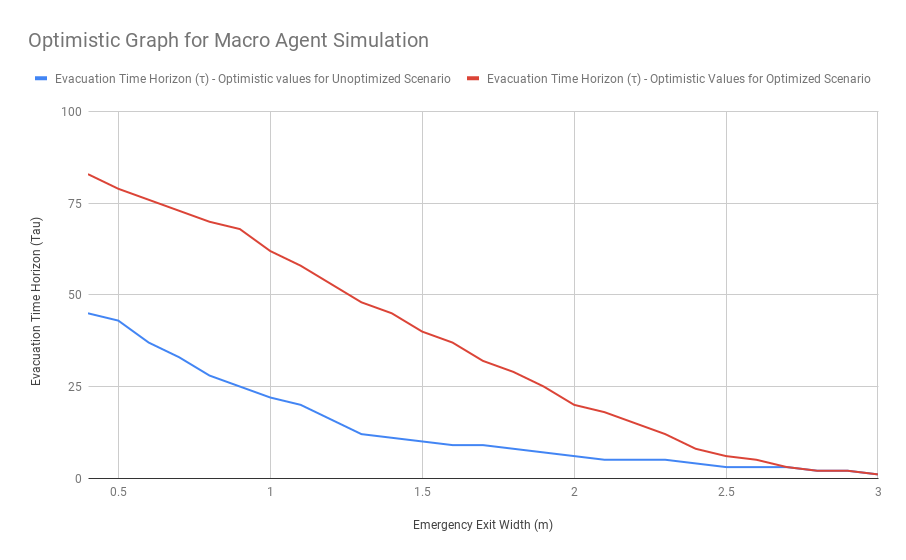
\includegraphics[scale=0.45]{simulation/Optimistic_Graph_for_Macro_Agent_Simulation.png}
  \caption{Optimistic Graph for Macro Agent Simulation}
  \label{Optimistic Graph for Macro Agent Simulation}
\end{figure}

\begin{figure}[H]
  \centering
  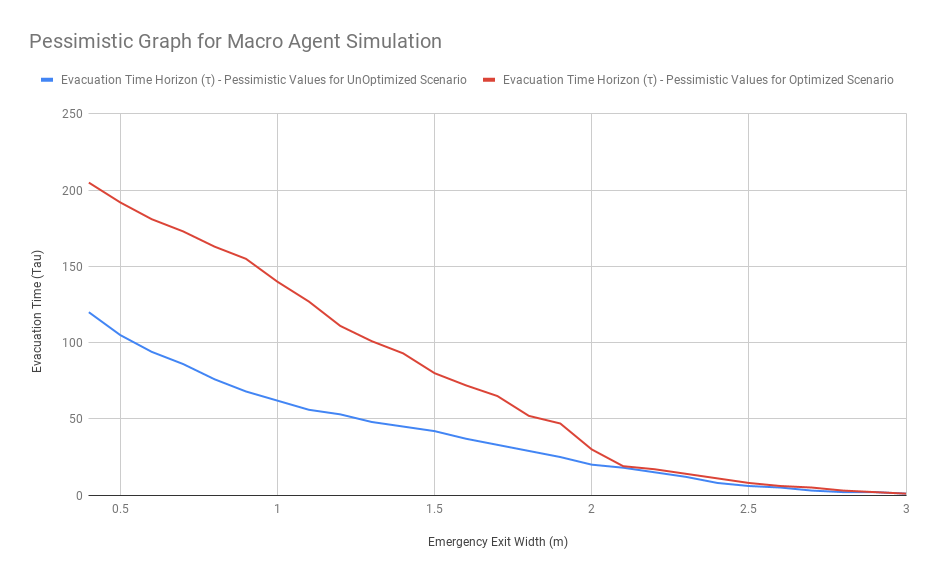
\includegraphics[scale=0.45]{simulation/Pessimistic_Graph_for_Macro_Agent_Simulation.png}
  \caption{Pessimistic Graph for Macro Agent Simulation}
  \label{Pessimistic Graph for Macro Agent Simulation}
\end{figure}

\begin{figure}[H]
  \centering
  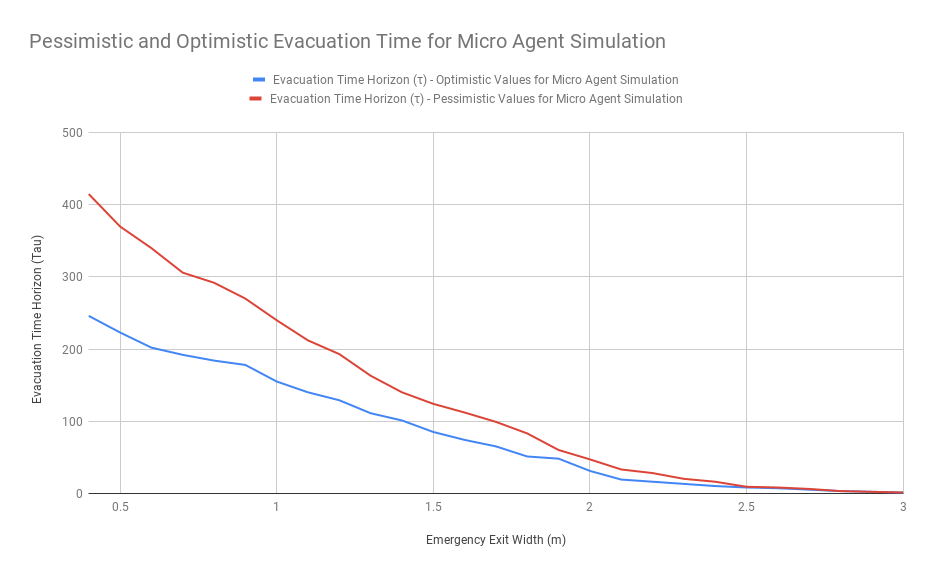
\includegraphics[scale=0.45]{simulation/Pessimistic_and_Optimistic_Evacuation_Time_for_Micro_Agent_Simulation.png}
  \caption{Pessimistic and Optimistic Evacuation Time for Micro Agent Simulation}
  \label{Pessimistic and Optimistic Evacuation Time for Micro Agent Simulation}
\end{figure}

\begin{figure}[H]
  \centering
  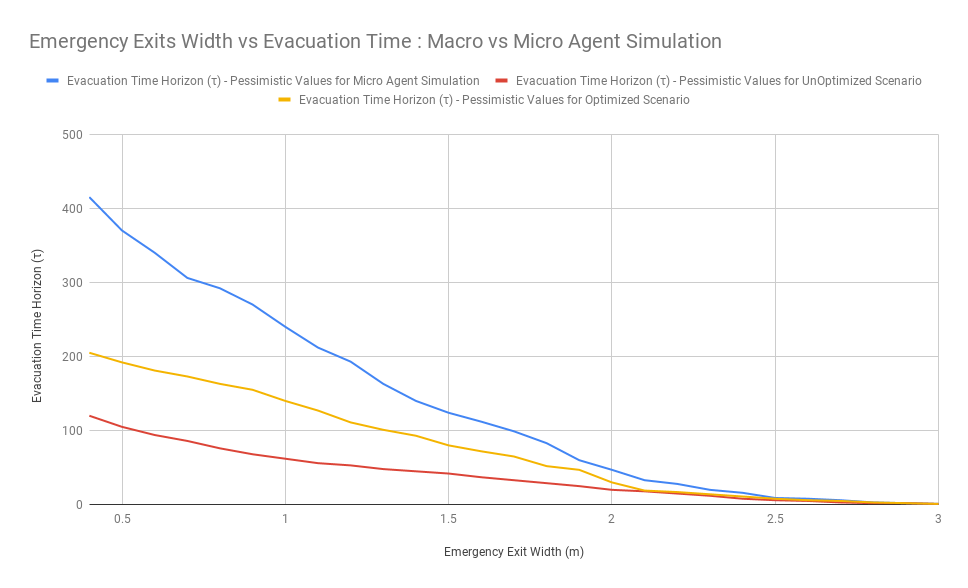
\includegraphics[scale=0.45]{simulation/summary.png}
  \caption{Emergency Exits Width vs Evacuation Time : Macro vs Micro Agent Simulation}
  \label{Emergency Exits Width vs Evacuation Time : Macro vs Micro Agent Simulation}
\end{figure}

From the above figures, it is made abundantly clear that the shorter the exits, the more time it would take for the evacuees to evacuate during a disaster scenario. Though this seems like a trivial scenario to depict, it has some serious implications. The most important inference that can be made from the presented data is the derivation of how many people can effectively navigate through to an exit during a disaster scenario. The presented scenario compares the obtained statistical data to the reference figure 8 from \cite{ref5}.

It is also made clear that with more constraints and more realism, the statistical data shows that the congestion tends to increase as the evacuees tend to take longer and longer time to evacuate. Especially in the final scenario with the pessimistic values denoted for the micro model agent simulation, the evacuation time required to get all the agents to safety is exponential compared to the previous cases. The difference between pessimistic case and the optimal one is that in the optimistic case, only the shortest possible path towards the exit is considered. However, for the pessimistic case, all possible exit strategies are considered and hence the pessimistic case scenario should be considered whilst modeling a safe topology that caters for safe exit paths.

It should also be mentioned that the social distances in the micro agent simulations are set according to the \href{https://www.gov.uk/workplace-fire-safety-your-responsibilities}{UK fire safety regulations} and the correponding guide given \href{https://www.merseyfire.gov.uk/aspx/pages/protection/pdf/Calculating_Occupancy_assembly_buildings_GT.pdf}{here}. The guide specifies that the maximum allowed density is 0.3 square meters per person, 0.5 for public houses, 0.8 for exhibition spaces, 1.0 for dining and 2.0 for sports areas etc. From \cite{ref5}, who also follows the same regulations, 1.25 persons per square meter is considered. Hence for this scenario, the social distances constraint is set accordingly. The area capacity constraints that are set throughout all these experiments are set according to these regulation standards. In our case, since its clearly mentioned that not more 6 are allowed within an office space, each room cannot hold more than 6 people at a single time.

Figure \ref{Emergency Exits Width vs Evacuation Time : Macro vs Micro Agent Simulation} presents a summary of all the congestion scenarios. The pessimistic values that are obtained from the micro agent scenario shows the difference in the exponentiation graphs where the time taken for evacuation exponentially increases with a time complexity of $O(N^3)$ as the width of the exits are decreased.  

\subsection{Case 4: Shortest Path vs Ideal Path}
\label{sec: Case 4: Shortest Path vs Ideal Path}

This section presents the evacuation of agents and the time required based on the scenario of shortest path and the ideal paths. The shortest path in realistic scenario may not always be the shortest time path. Hence it is required to re-route the agents to a more optimal path, i.e. the ideal path in order to reach the exit points. In order to identify the ideal path, the algorithm traveses through all possible paths from the given agent location and then based on flow capacity and congestion ratio, it strategizes an ideal path for the agents to take whilst heading towards the safe zone. 

The ideal path formation depends on some factors which are given below:

\begin{itemize}
  \item Number of people in the group - this is used in calculation of the ideal path as the number of people in a group can be used to determine if other cluster of agents can form a congestion or not. It falls under congestion control and prediction.
  \item The movement speed of the group - this is used to calculate the ideal path by predicting if the group can reach a certain location or not to avoid congestion and cluster, if the group can access for instance an emergency service like elevators, emergency stairwells, exits etc.
  \item Area capacity - This is used to determine if the agent(s) are to be re-routed to another path.
  \item Door and cell flow dynamic- cell flow dynamic is used to determine if the stream of agents can be navigated through or not, to determine if a certain pathway is one way navigation only or not. The door flow capacity is used to determine the queuing and wait time as most congestions occur at key door and exit points. 
\end{itemize}

The above mentioned conditions are incorporated in this scenario in order to scan through all the possible paths and then determine an ideal path for the agents. Since walking speeds play an important role in determining routing path, it became a necessity to group people according to \textit{Energetic consequences of human sociality: walking speed choices among friendly dyads} by Wagnild et al. \cite{ref24}. According to Wagnild male agents walk at a faster pace when they are alone at an average speed of 1.53 $m/s$. They walk the fastest with a male companion at a speed of 1.60 $m/s$. The speed is subsequently lowered in the presence of a female agent to match her speed, which comes to around 1.44 $m/s$. Females walk even slower when accompanied with a female partner at a speed of 1.39 $m/s$. 

The mentioned walking speeds are done so in order to account for the expense of calories spent whilst walking. Men tend to reduce their speeds while walking with a female partner, female agents similarly increase their speeds and the compromized speed averaging at 1.44 $m/s$ is set upon. All the agents presented in the study are capable adults with no apparent health problems. 

However in order to make a realistic approach to simulation, all age groups should be considered. Hence for this case, 20\% of the total number of agents are considered agents with slower movement speeds, i.e., between 0.7 $m/s$ and 1.2 $m/s$. All the other agents are given a random speed between 1.2 and 1.6 $m/s$. The door flow capacity is set to not more than 5 for pessimistic cases as the same value has been used in \cite{ref5}, to remain coherent with the statistics. The upper limit, i.e. optimistic value is no more than 16 persons can pass through a 1 meter wide door during one time slot $\tau$. 

In order to model the exact movement speed of an agent within the PedSim environment, the total time required to move an agent across the entire breadth of the topology recorded and then subsequently divided by the total time taken in order to calculate the average speed that is taken by the agent to traverse 1 $m$ of the topology. This then can be used to set variable speeds according to aforementioned constraints and then the scenario is run within the environment of PedSim. The following graphs depict the pessimistic and the optimistic values that are obtained as a result of the simulations. However, for macro agent scenario, a movement speed based on the normal distribution across all agents is set.

The observational data from \cite{ref5} is used as a baseline reference in order to conduct the forthcoming simulations. The study is presented as follows:

\begin{figure}[H]
  \centering
  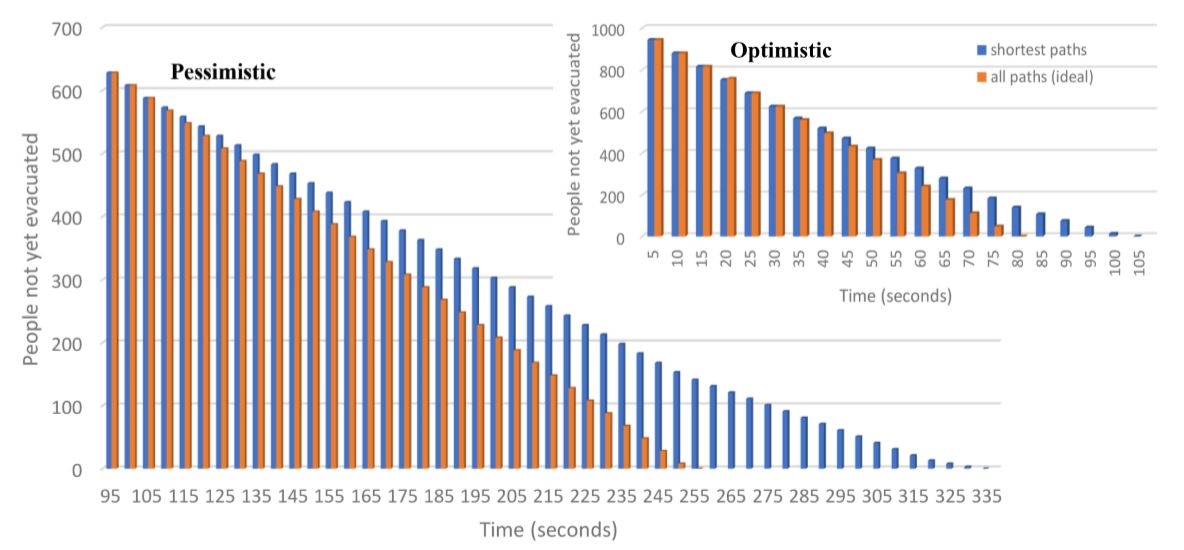
\includegraphics[scale=0.5]{simulation/ideal_evacuation_along_shortest_paths.JPG}
  \caption{Ideal Evacuation vs Shortest Path Evacuation Along Shortest Path for Macro Agents}
  \label{Ideal Evacuation vs Shortest Path Evacuation Along Shortest Path for Macro Agents}
\end{figure}

The above figure represents the number of people who can be evacuated within the given time frame for both pessimistic and optimistic cases, while simulating the whole scene for macro agent scenario. The pessimistic scenario runs for a total of 5 minutes and 35 seconds while the optimistic scenario runs for a total of 1 minute and 20 seconds. The figure below depict the cases for optimistic scenario that run on an macro agent model simulating an optimized algorithm for path routing.

\begin{figure}[H]
  \centering
  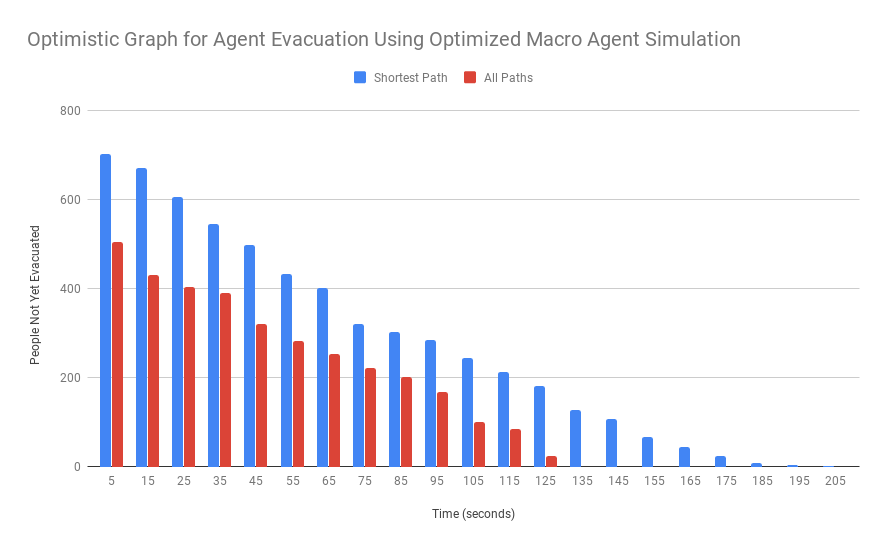
\includegraphics[scale=0.5]{simulation/Optimistic_Macro.png}
  \caption{Optimistic Graph for Agent Evacuation Using Optimized Macro Agent Simulation}
  \label{Optimistic Graph for Agent Evacuation Using Optimized Macro Agent Simulation}
\end{figure}

Compared to the previous figure \ref{Ideal Evacuation vs Shortest Path Evacuation Along Shortest Path for Macro Agents} depicting the optimistic scenario, its immediately evident that evacuation required is longer compared to and the number of agents that are not evacuated stays on for a longer period of time. This is with an increased capacity for the pathways since its the optimal scenario. The simulation takes a total of 3 minutes and 15 seconds in order to evacuate all people to safety. Some of the inferences made are as follows:

\begin{itemize}
  \item The interesting result to note is at the end tails of both the graphs. The graph from figure \ref{Ideal Evacuation vs Shortest Path Evacuation Along Shortest Path for Macro Agents} shows that the agents that follow the shortest paths tend to be evacuated last compared to the agents that follow the ideal path scenario based on the computation of all path.
  \item In the optimized macro agent case however, we observe that there is a shift from this pattern of behavior as agents that follow either path strategy have similar evacuation times. 
  \item This is due to the fact that, in the results provided in \ref{Ideal Evacuation vs Shortest Path Evacuation Along Shortest Path for Macro Agents}, the agents flow plainly till the third of the total evacuation time and then the agents that follow the shortest path strategy start to experience congestion, while the agents that follow all paths strategy can evacuate quicker.
  \item This phenomenon is not experienced in the presented optimized macro agent scenario as depicted in \ref{Optimistic Graph for Agent Evacuation Using Optimized Macro Agent Simulation} as the computation time required for both shortest path and ideal paths are the same for very low number of agents and hence for very low number of agents the evacuation time required is similar.
  \item This however becomes very different for very large number of agents and as it can be seen from the graph \ref{Optimistic Graph for Agent Evacuation Using Optimized Macro Agent Simulation}, the curve becomes exponential ($O(N^2)$), for the all paths strategy and increases steadily as the number of agents increase.
\end{itemize}

The next step is to compare the differences in scaling between the pessimistic case for  macro agent model simulated using the unoptimized algorithm and the pessmisictic case for macro agent model running on the optimized algorithm. The prediction is that the rates of scaling will be very drastic as the pessimistic case reduces the flow capacity and also considers a few of the exits blocked. For the purposes of this experiment it was assumed that 2 out of 4 exits were blocked due to a static emergency like earthquake and hence the agents have to be re-routed to safety through the other exit points. This case is particularly interesting as congestions can be observed and how the agents tackle these congestions through predictive re-routing can be observed. 

The next figure \ref{Pessimistic Graph for Agent Evacuation Using Optimized Macro Agent Simulation} presents the aforementioned case.

\begin{figure}[H]
  \centering
  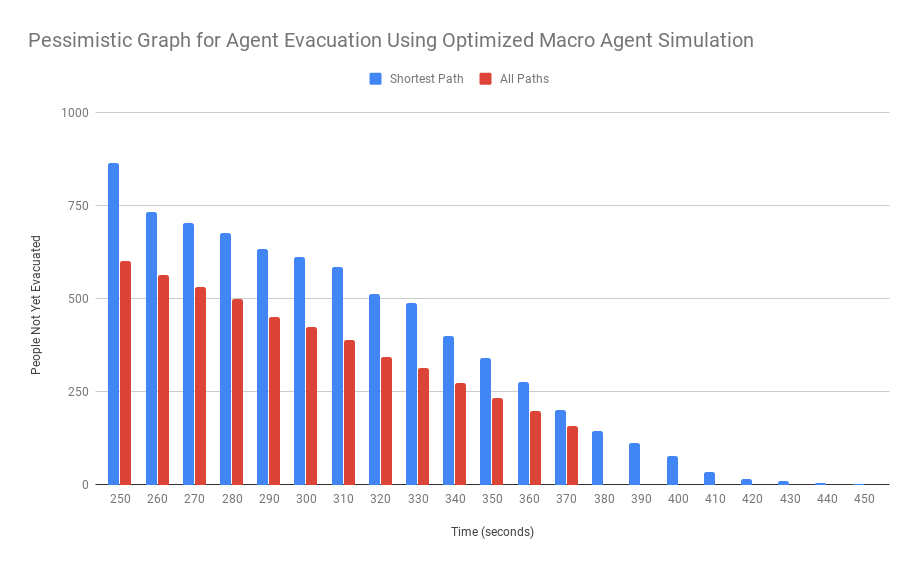
\includegraphics[scale=0.5]{simulation/Pessimistic_Macro.png}
  \caption{Pessimistic Graph for Agent Evacuation Using Optimized Macro Agent Simulation}
  \label{Pessimistic Graph for Agent Evacuation Using Optimized Macro Agent Simulation}
\end{figure}


The above represented graph typically confirms the previously described hypothesis in terms of scaling. As it can be observed quite clearly, the time required for the evacuation of agents in comparison to the figure \ref{Ideal Evacuation vs Evacuation Along Shortest Path for Macro Agents} is almost 1.5 times the time required for the evacuation for the same case presented.

The following are some inferences that are derived from the above graph:

\begin{itemize}
  \item Evidently the tail end of the graph for agents following the all paths strategy raises exponentially ($O(N^2)$)
  \item The agents following the shortest paths strategy only increase linearly as the number of agents increase.
  \item The implications of these scaling differences are especially important as it can be further broken and analyzed as to which of the constraints cause this peak in scaling. Upon further investigation into the particular constraint causing the computation time difference, it is found that changing the values of area capacity and flow capacity makes most of the difference.
\end{itemize}

The next two cases present the optimistic and the pessimistic cases of the micro agent model scenario.

\begin{figure}[H]
  \centering
  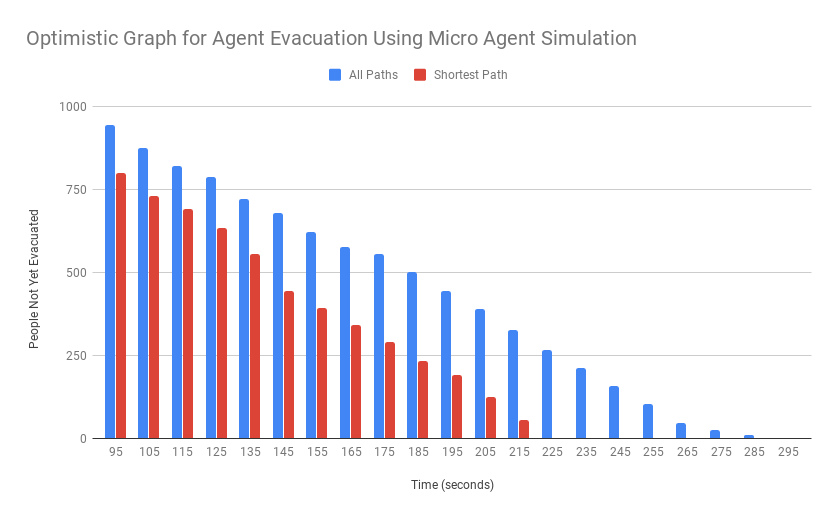
\includegraphics[scale=0.5]{simulation/Optimistic_Micro.png}
  \caption{Optimistic Case for Ideal Evacuation vs Shortest Path Evacuation Along Shortest Path for Micro Agents}
  \label{Optimistic Case for Ideal Evacuation vs Shortest Path Evacuation Along Shortest Path for Micro Agents}
\end{figure}

The figure given above depicts an interesting scenario compared to its counter part - the pessimistic case as presented in \ref{Ideal Evacuation vs Shortest Path Evacuation Along Shortest Path for Macro Agents}. Inferences from the given diagram will be presented below while discussing the following figure.

\begin{figure}[H]
  \centering
  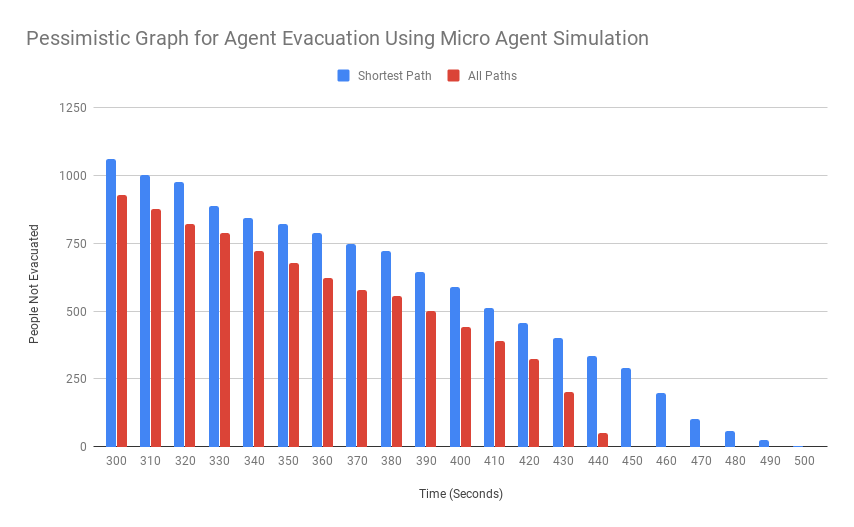
\includegraphics[scale=0.5]{simulation/Pessimistic_Micro.png}
  \caption{Pessimistic Case for Ideal Evacuation vs Shortest Path Evacuation Along Shortest Path for Micro Agents}
  \label{Pessimistic Case for Ideal Evacuation vs Shortest Path Evacuation Along Shortest Path for Micro Agents}
\end{figure}


The above two figures depict the interesting differences between the macro and micro agent simulation. As it can be observed from the figures \ref{Optimistic Case for Ideal Evacuation vs Shortest Path Evacuation Along Shortest Path for Micro Agents} and \ref{Pessimistic Case for Ideal Evacuation vs Shortest Path Evacuation Along Shortest Path for Micro Agents}, it takes longer than the macro agent model simulation in order to evacuate all the people to safety. The following inferences are presented in brief to compare and constrast between the obtained results:


\begin{itemize}
  \item It is interesting to note the opposite effect that occurs in \ref{Optimistic Case for Ideal Evacuation vs Shortest Path Evacuation Along Shortest Path for Micro Agents} when compared to the results obtained from the optimistic case presented in the figure \ref{Ideal Evacuation vs Shortest Path Evacuation Along Shortest Path for Macro Agents}.
  \item In an optimistic scenario, due to higher capacity and a higher degree of resulting congestion avoidance, the shortest path algorithm functions more optimally compared to the all paths strategy.
  \item This however becomes a more or less even total evacuation time as shown in figure \ref{Pessimistic Case for Ideal Evacuation vs Shortest Path Evacuation Along Shortest Path for Micro Agents}. The contrast in the evacuation time occurs due to the following reason:
    \begin{itemize}
      \item During a pessimistic scenario, it is assumed that 50\% of the total emergency exits are inaccessible due to a static emergency blockade. Hence as the numbers dwindle the time differnence between shortest paths and the all paths strategy becomes one and the same. Hence this causes the noticeable difference between the two results given above. 
    \end{itemize}
\end{itemize}

In summary it can drawn to a conclusion that the micro agent simulation with the all paths strategy takes the highest amount of time to evacuate, exhibiting a time complexity of $O(N^3)$. The macro agent model with the optimized algorithm takes a running time of $O(N^2)$.
